
\documentclass[letterpaper,hide notes,xcolor={table,svgnames},pdftex,10pt]{beamer}
\def\showexamples{t}

\usecolortheme{crane}
\setbeamertemplate{navigation symbols}{}

\usetheme{MyPittsburgh}
\usepackage{hyperref}
\usepackage{graphicx,xspace}
\usepackage[normalem]{ulem}
\usepackage{multicol}
\usepackage{amsmath,amssymb,amsthm,graphicx,xspace}
\newcommand\SF[1]{$\bigstar$\footnote{SF: #1}}

\usepackage[sfdefault,lf]{carlito}
\usepackage[T1]{fontenc}
\usepackage[scaled]{beramono}
\usepackage{tikzpagenodes}
\newcommand{\Rplus}{\protect\hspace{-.1em}\protect\raisebox{.35ex}{\small{\small\textbf{+}}}}
\newcommand{\Cpp}{\mbox{C\Rplus\Rplus}\xspace}

\newcounter{tmpnumSlide}
\newcounter{tmpnumNote}

\newcommand\mnote[1]{%
	\addtocounter{tmpnumSlide}{1}
	\ifdefined\showcues {~\tiny\fbox{\arabic{tmpnumSlide}}}\fi
	\note{\setlength{\parskip}{1ex}\addtocounter{tmpnumNote}{1}\textbf{\Large \arabic{tmpnumNote}:} {#1\par}}}

\newcommand\mmnote[1]{\note{\setlength{\parskip}{1ex}#1\par}}


\newcommand\mquestion[2]{{~\color{red}\fbox{?}}\note{\setlength{\parskip}{1ex}\par{\Large \textbf{?}} #1} \note{\setlength{\parskip}{1ex}\par{\Large \textbf{A}} #2\par}\ifdefined \presentationonly \pause \fi}

\newcommand\blackboard[1]{%
	\ifdefined   \showblackboard
		{#1}
	\else {\begin{center} \fbox{\colorbox{blue!30}{%
						\begin{minipage}{.95\linewidth}%
							\hspace{\stretch{1}} Some space intentionally left blank; done at the blackboard.%
						\end{minipage}}}\end{center}}%
	\fi%
}

\usepackage{listings}
\lstset{%
	keywordstyle=\bfseries,
	aboveskip=15pt,
	belowskip=15pt,
	captionpos=b,
	identifierstyle=\ttfamily,
	frame=lines,
	numbers=left, basicstyle=\scriptsize, numberstyle=\tiny, stepnumber=0, numbersep=2pt}

\usepackage{siunitx}
\newcommand\sius[1]{\num[group-separator = {,}]{#1}\si{\micro\second}}
\newcommand\sims[1]{\num[group-separator = {,}]{#1}\si{\milli\second}}
\newcommand\sins[1]{\num[group-separator = {,}]{#1}\si{\nano\second}}
\sisetup{group-separator = {,}, group-digits = true}

%% -------------------- tikz --------------------
\usepackage{tikz}
\usetikzlibrary{positioning}
\usetikzlibrary{arrows,backgrounds,automata,decorations.shapes,decorations.pathmorphing,decorations.markings,decorations.text}

\tikzstyle{place}=[circle,draw=blue!50,fill=blue!20,thick, inner sep=0pt,minimum size=6mm]
\tikzstyle{transition}=[rectangle,draw=black!50,fill=black!20,thick, inner sep=0pt,minimum size=4mm]

\tikzstyle{block}=[rectangle,draw=black, thick, inner sep=5pt]
\tikzstyle{bullet}=[circle,draw=black, fill=black, thin, inner sep=2pt]

\tikzstyle{pre}=[<-,shorten <=1pt,>=stealth',semithick]
\tikzstyle{post}=[->,shorten >=1pt,>=stealth',semithick]
\tikzstyle{bi}=[<->,shorten >=1pt,shorten <=1pt, >=stealth',semithick]

\tikzstyle{mut}=[-,>=stealth',semithick]

\tikzstyle{treereset}=[dashed,->, shorten >=1pt,>=stealth',thin]

\usepackage{ifmtarg}
\usepackage{xifthen}
\makeatletter
% new counter to now which frame it is within the sequence
\newcounter{multiframecounter}
% initialize buffer for previously used frame title
\gdef\lastframetitle{\textit{undefined}}
% new environment for a multi-frame
\newenvironment{multiframe}[1][]{%
	\ifthenelse{\isempty{#1}}{%
		% if no frame title was set via optional parameter,
		% only increase sequence counter by 1
		\addtocounter{multiframecounter}{1}%
	}{%
		% new frame title has been provided, thus
		% reset sequence counter to 1 and buffer frame title for later use
		\setcounter{multiframecounter}{1}%
		\gdef\lastframetitle{#1}%
	}%
	% start conventional frame environment and
	% automatically set frame title followed by sequence counter
	\begin{frame}%
		\frametitle{\lastframetitle~{\normalfont(\arabic{multiframecounter})}}%
		}{%
	\end{frame}%
}
\makeatother

\makeatletter
\newdimen\tu@tmpa%
\newdimen\ydiffl%
\newdimen\xdiffl%
\newcommand\ydiff[2]{%
	\coordinate (tmpnamea) at (#1);%
	\coordinate (tmpnameb) at (#2);%
	\pgfextracty{\tu@tmpa}{\pgfpointanchor{tmpnamea}{center}}%
	\pgfextracty{\ydiffl}{\pgfpointanchor{tmpnameb}{center}}%
	\advance\ydiffl by -\tu@tmpa%
}
\newcommand\xdiff[2]{%
	\coordinate (tmpnamea) at (#1);%
	\coordinate (tmpnameb) at (#2);%
	\pgfextractx{\tu@tmpa}{\pgfpointanchor{tmpnamea}{center}}%
	\pgfextractx{\xdiffl}{\pgfpointanchor{tmpnameb}{center}}%
	\advance\xdiffl by -\tu@tmpa%
}
\makeatother
\newcommand{\copyrightbox}[3][r]{%
	\begin{tikzpicture}%
		\node[inner sep=0pt,minimum size=2em](ciimage){#2};
		\usefont{OT1}{phv}{n}{n}\fontsize{4}{4}\selectfont
		\ydiff{ciimage.south}{ciimage.north}
		\xdiff{ciimage.west}{ciimage.east}
		\ifthenelse{\equal{#1}{r}}{%
			\node[inner sep=0pt,right=1ex of ciimage.south east,anchor=north west,rotate=90]%
			{\raggedleft\color{black!50}\parbox{\the\ydiffl}{\raggedright{}#3}};%
		}{%
			\ifthenelse{\equal{#1}{l}}{%
				\node[inner sep=0pt,right=1ex of ciimage.south west,anchor=south west,rotate=90]%
				{\raggedleft\color{black!50}\parbox{\the\ydiffl}{\raggedright{}#3}};%
			}{%
				\node[inner sep=0pt,below=1ex of ciimage.south west,anchor=north west]%
				{\raggedleft\color{black!50}\parbox{\the\xdiffl}{\raggedright{}#3}};%
			}
		}
	\end{tikzpicture}
}


%% --------------------

%\usepackage[excludeor]{everyhook}
%\PushPreHook{par}{\setbox0=\lastbox\llap{MUH}}\box0}

%\vspace*{\stretch{1}

%\setbox0=\lastbox \llap{\textbullet\enskip}\box0}

\setlength{\parskip}{\fill}

\newcommand\noskips{\setlength{\parskip}{1ex}}
\newcommand\doskips{\setlength{\parskip}{\fill}}

\newcommand\xx{\par\vspace*{\stretch{1}}\par}
\newcommand\xxs{\par\vspace*{2ex}\par}
\newcommand\tuple[1]{\langle #1 \rangle}
\newcommand\code[1]{{\sf \footnotesize #1}}
\newcommand\ex[1]{\uline{Example:} \ifdefined \presentationonly \pause \fi
	\ifdefined\showexamples#1\xspace\else{\uline{\hspace*{2cm}}}\fi}

\newcommand\ceil[1]{\lceil #1 \rceil}


\AtBeginSection[]
{
	\begin{frame}
		\frametitle{Outline}
		\tableofcontents[currentsection]
	\end{frame}
}



\pgfdeclarelayer{edgelayer}
\pgfdeclarelayer{nodelayer}
\pgfsetlayers{edgelayer,nodelayer,main}

\tikzstyle{none}=[inner sep=0pt]
\tikzstyle{rn}=[circle,fill=Red,draw=Black,line width=0.8 pt]
\tikzstyle{gn}=[circle,fill=Lime,draw=Black,line width=0.8 pt]
\tikzstyle{yn}=[circle,fill=Yellow,draw=Black,line width=0.8 pt]
\tikzstyle{empty}=[circle,fill=White,draw=Black]
\tikzstyle{bw} = [rectangle, draw, fill=blue!20,
text width=4em, text centered, rounded corners, minimum height=2em]

\newcommand{\CcNote}[1]{% longname
	This work is licensed under the \textit{Creative Commons #1 3.0 License}.%
}
\newcommand{\CcImageBy}[1]{%
	\includegraphics[scale=#1]{creative_commons/cc_by_30.pdf}%
}
\newcommand{\CcImageSa}[1]{%
	\includegraphics[scale=#1]{creative_commons/cc_sa_30.pdf}%
}
\newcommand{\CcImageNc}[1]{%
	\includegraphics[scale=#1]{creative_commons/cc_nc_30.pdf}%
}
\newcommand{\CcGroupBySa}[2]{% zoom, gap
	\CcImageBy{#1}\hspace*{#2}\CcImageNc{#1}\hspace*{#2}\CcImageSa{#1}%
}
\newcommand{\CcLongnameByNcSa}{Attribution-NonCommercial-ShareAlike}

\newenvironment{changemargin}[1]{% 
	\begin{list}{}{% 
		\setlength{\topsep}{0pt}% 
		\setlength{\leftmargin}{#1}% 
		\setlength{\rightmargin}{1em}
		\setlength{\listparindent}{\parindent}% 
		\setlength{\itemindent}{\parindent}% 
		      \setlength{\parsep}{\parskip}% 
		      }% 
		\item[]}{\end{list}}




\title{Lecture 10 --- Pipes and Shared Memory}

\author{Jeff Zarnett \\ \small \texttt{jzarnett@uwaterloo.ca}}
\institute{Department of Electrical and Computer Engineering \\
	University of Waterloo}
\date{\today}


\begin{document}

\begin{frame}
	\titlepage

\end{frame}

\begin{frame}
	\frametitle{More IPC}

	In addition to message passing, we should talk about pipes and shared memory.


\end{frame}


\begin{frame}
	\frametitle{UNIX Pipes}

	In UNIX, we can create a \textit{pipe} to set up communication.

	\begin{center}
		
\includegraphics[width=0.7\textwidth]{images/mario-pipe.jpg}
	\end{center}

\end{frame}

\begin{frame}
	\frametitle{UNIX Pipes}




	The producer writes in one end; the consumer receives on the other.

	This is unidirectional, so if bidirectional communication is desired, two pipes must be used (going in different directions).

\end{frame}

\begin{frame}
	\frametitle{Constructing a UNIX Pipe}

	The method is \texttt{pipe} and it is constructed with the call: \\
	\texttt{pipe( int fileDescriptors[])}\\
	\quad where \texttt{fileDescriptors[0]} is the read-end; and\\
	\quad \texttt{fileDescriptors[1]} is the write-end.

	Yes, \texttt{fileDescriptors} means that UNIX thinks of a pipe as a file\\
	\quad even though it is in memory.


\end{frame}

\begin{frame}
	\frametitle{UNIX Pipes}

	\begin{center}
		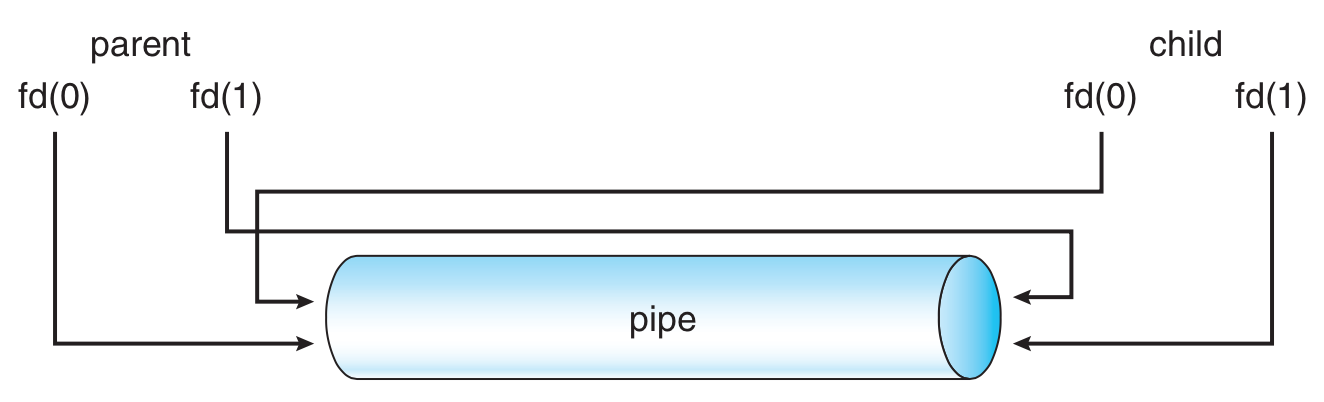
\includegraphics[width=0.9\textwidth]{images/unix-pipe.png}
	\end{center}

\end{frame}

\begin{frame}
	\frametitle{UNIX Pipes}

	The pipe is a block of main memory interpreted as a circular queue.

	Each entry in the queue is fixed in size and usually one character.

	The sender may place the message into the queue in small chunks.

	The receiver gets data one character at a time.

	The sender and receiver need to know when the message is finished.

	Solutions: termination character, or declared length at the start.

\end{frame}

\begin{frame}
	\frametitle{Named Pipes}

	A UNIX pipe may be stored on disk.

	When this happens, we call it a \alert{named pipe}.

	Unless we make it a named pipe, a pipe exists only as long as the processes are communicating.

	Regular pipes require a parent-child process relationship.\\
	\quad Named pipes do not.

	Named pipes are also bidirectional, but one direction at a time.

\end{frame}

\begin{frame}
	\frametitle{UNIX Command Line Pipes}

	You may have worked with pipes on the UNIX command line.

	A command like \texttt{ cat fork.c | less } creates a pipe;.

	It takes the output of the \texttt{cat} program and delivers it as input to \texttt{less}.

\end{frame}

\begin{frame}[fragile]
	\frametitle{Pipe Code Example}

	Use \texttt{fork} to spawn a new child process and then setting up a communication pipe between the parent and child.

	We will send a message ``Greetings'' from the parent to the child.

	\begin{lstlisting}[language=C]

  char write_msg[BUFFER_SIZE] = "Greetings"; 
  char read_msg[BUFFER_SIZE];
  int fd[2];
  pid_t pid;

  if (pipe(fd) == -1) {
    fprintf(stderr,"Pipe failed");
    return 1;
  }

\end{lstlisting}


\end{frame}

\begin{frame}[fragile]
	\frametitle{Pipe Code Example, Continued}

	\begin{lstlisting}[language=C]

/* fork a child process */
  pid = fork();
  
  if (pid < 0) { 
    /* error occurred */ 
    fprintf(stderr, "Fork Failed"); 
    return 1;
  }
 if (pid > 0) { /* parent process */
    /* close the unused end of the pipe */ 
    close(fd[READ_END]);
    
    /* write to the pipe */
    write(fd[WRITE_END], write_msg, strlen(write_msg)+1);
    
    /* close the write end of the pipe */
    close(fd[WRITE_END]);
    
  } 

\end{lstlisting}

	\texttt{READ\_END} is defined as \texttt{0} in a \texttt{\#define} directive.\\
	\texttt{WRITE\_END} is defined as \texttt{1} in a \texttt{\#define} directive.

\end{frame}

\begin{frame}[fragile]
	\frametitle{Pipe Code Example, Continued}


	\begin{lstlisting}[language=C]
  else { /* child process */
    /* close the unused end of the pipe */ 
    close(fd[WRITE_END]);
    
    /* read from the pipe */
    read(fd[READ_END], read_msg, BUFFER_SIZE); 
    printf("read %s",read_msg);
     /* close the write end of the pipe */
     close(fd[READ_END]); 
  }
  return 0;
}
\end{lstlisting}

	Does the output match what's supposed to happen?

	Or are there extra characters?

\end{frame}

\begin{frame}
	\frametitle{Creating a Named Pipe}

	If we wanted to create a named pipe, the system call is \texttt{mkfifo}.

	Sometimes a named pipe is called a FIFO.

	As it is a file, it can be manipulated with the usual UNIX file system calls: \texttt{open}, \texttt{read}, \texttt{write}, and \texttt{close}.

\end{frame}


\begin{frame}
	\frametitle{Shared Memory}

	Conceptually, the idea of shared memory is very simple.

	A particular region of memory is designated as being shared between multiple processes, all of whom may read and write to that location.

	To share an area of memory, the OS must be notified.

\end{frame}


\begin{frame}
	\frametitle{What's yours is mine...}

	Normally, a region of memory is associated with exactly one process (its owner).


	\begin{center}
		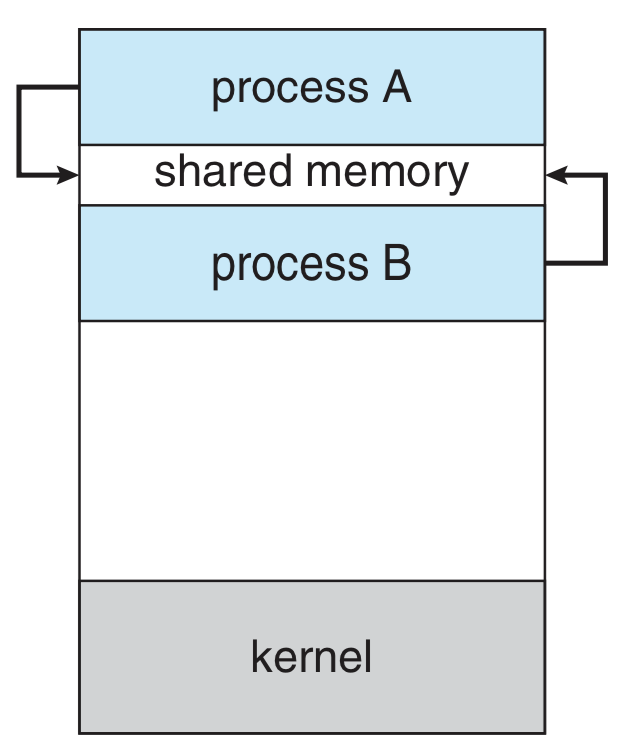
\includegraphics[width=0.4\textwidth]{images/shared-memory.png}
	\end{center}

	The kernel is only involved in the setup and cleanup of that shared area.

\end{frame}


\begin{frame}
	\frametitle{Whose Turn Is It Anyway?}

	When a section of memory is shared, there exists the possibility that one process will overwrite another's changes.

	To prevent this sort of problem, we will need a mechanism for co-ordination...

	A subject we will return to later.

\end{frame}


\begin{frame}[fragile]
	\frametitle{Share a Key}

	Suppose we want to share a section of memory.

	We need to obtain a \alert{key} that identifies a specific memory segment.

	Keys are just integer values, so we would like them to be unique.

	One method is to generate the key with the ``file to key'' function found in \texttt{sys/ipc.h}:
	\begin{lstlisting}[language=C]
key_t ftok( char *pathname, int proj )
\end{lstlisting}

	The key is generated from the given file name (\texttt{pathname}) and the value \texttt{proj}.

\end{frame}


\begin{frame}
	\frametitle{Not Private Key Encryption}

	There is a very small risk of duplicate numbers.

	Another way we can get a key is using the constant \texttt{IPC\_PRIVATE}.

	If we give the constant in where a \texttt{key\_t} is expected then a guaranteed unique key is returned.

\end{frame}


\begin{frame}
	\frametitle{Workflow for Shared Memory}

	\begin{itemize}
		\item Create a new shared memory segment -- \texttt{shmget}.
		\item Attach the shared memory segment -- \texttt{shmat}.
		\item Then the process can use the shared memory.
		\item Detach -- \texttt{shmdt}.
		\item Delete the shared memory segment, done by one process only -- \texttt{shmctl}.
	\end{itemize}

\end{frame}


\begin{frame}[fragile]
	\frametitle{Create}

	To create a shared memory segment, or get a reference to an existing one, we use \texttt{shmget}.

	\begin{lstlisting}[language=C]
int shmget( key_t key, size_t size, int shmflg );
\end{lstlisting}

	The first argument is the key, which can be either the result of a \texttt{ftok()} call or the constant \texttt{IPC\_PRIVATE}.

	\texttt{size}: how many bytes of memory are to be shared.

	\texttt{shmflg}: access permissions (UNIX standards, eg 600)\\
	\quad Optional: \texttt{IPC\_CREAT}, \texttt{IPC\_EXCL}

	Return value: the integer ID of the shared memory segment.
\end{frame}

\begin{frame}[fragile]
	\frametitle{Attach}
	\begin{lstlisting}[language=C]
void* shmat( int shmid, const void* shmaddr, int shmflg );
\end{lstlisting}

	\texttt{shmid}: ID of the shared memory segment.

	\texttt{shmaddr}: where it should go; always use \texttt{NULL}.

	\texttt{shmflg}: optionally, \texttt{SHM\_RDONLY}

	Return value: standard C pointer with the address of shared memory.

	But how do we know what the shared memory segment ID is?

\end{frame}

\begin{frame}
	\frametitle{This is the key for what?}

	If we created the segment ourselves, we obviously know where it is.

	But presumably you want some other process to have it as well.

	If two processes use the same input values for \texttt{ftok()} they will get the same result, so that's one method.

	Or, if a parent attaches a shared memory segment and then calls \texttt{fork()}, the child inherits the shared memory segments, so it's is already set up.


\end{frame}


\begin{frame}
	\frametitle{Detach Cable!}

	\begin{center}
		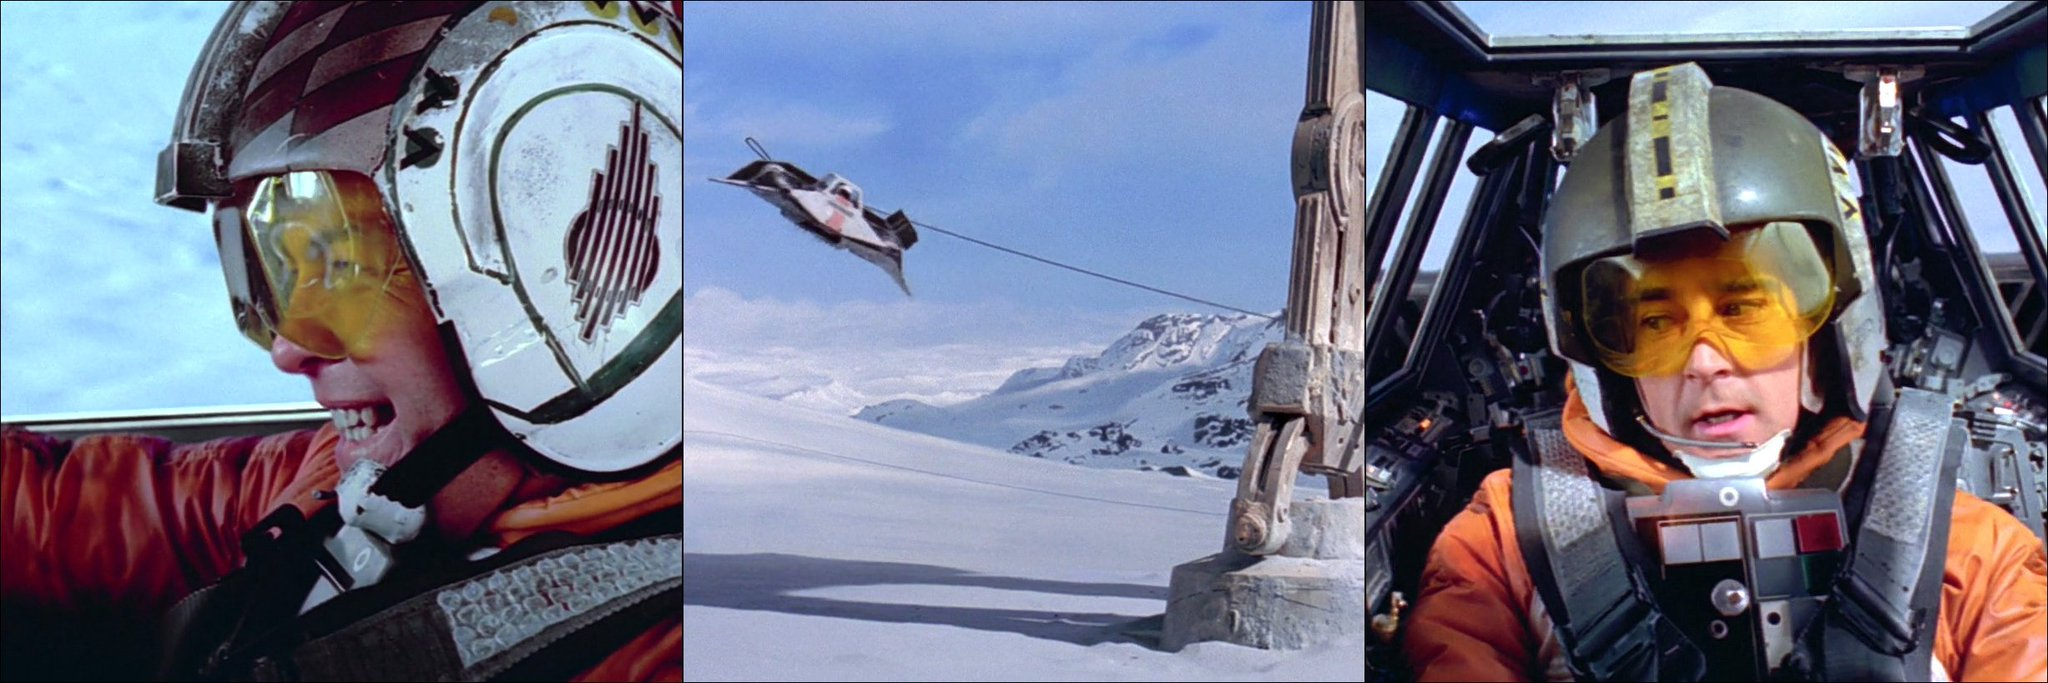
\includegraphics[width=0.9\textwidth]{images/detach-cable.jpg}
	\end{center}


\end{frame}

\begin{frame}[fragile]
	\frametitle{Detach Segment}

	When we are done with a segment we can detach from it with \texttt{shmdt}.

	\begin{lstlisting}[language=C]
int shmdt( const void* shmaddr );
\end{lstlisting}

	\texttt{shmaddr}: the address returned by the attach call

	If we forget, it happens at process termination (but don't forget!)
\end{frame}

\begin{frame}[fragile]
	\frametitle{Delete Shared Memory}
	\begin{lstlisting}[language=C]
int shmctl( int schmidt, int cmd, struct shmid_ds *buf )
\end{lstlisting}

	This function can do a lot more than delete it, such as modify properties of the data structure that is used to control shared memory.

	The command is  \texttt{IPC\_RMID} (``remove ID'').

	We must leave the last argument as \texttt{NULL} for this deletion.

	Deletion may be deferred!

\end{frame}


\begin{frame}[fragile]
	\frametitle{Shared Memory Example}
	\begin{lstlisting}[language=C]
#define _XOPEN_SOURCE
#include <stdio.h>
#include <stdlib.h>
#include <sys/shm.h>
#include <string.h>
#include <unistd.h>
#include <sys/wait.h>

int main( int argc, char** argv ) { 
    int shmid = shmget( IPC_PRIVATE, 32, IPC_CREAT | 0666  );  

    int pid = fork();
    if ( pid > 0 ) { /* Parent */
        waitpid( pid, NULL, 0 );
        void* mem = shmat( shmid, NULL, 0 );
        printf("The msg received from the child is %s.\n", (char*) mem );
        shmdt( mem );
        shmctl( shmid, IPC_RMID, NULL );
    } else if ( pid == 0 ) { /* Child */
        void* mem = shmat( shmid, NULL, 0 );
        memset( mem, 0, 32 );
        sprintf( mem, "Hello World" );
        shmdt( mem );
    }   
    return 0;
}
\end{lstlisting}


\end{frame}


\begin{frame}
	\frametitle{Consult the Map}

	\begin{center}
		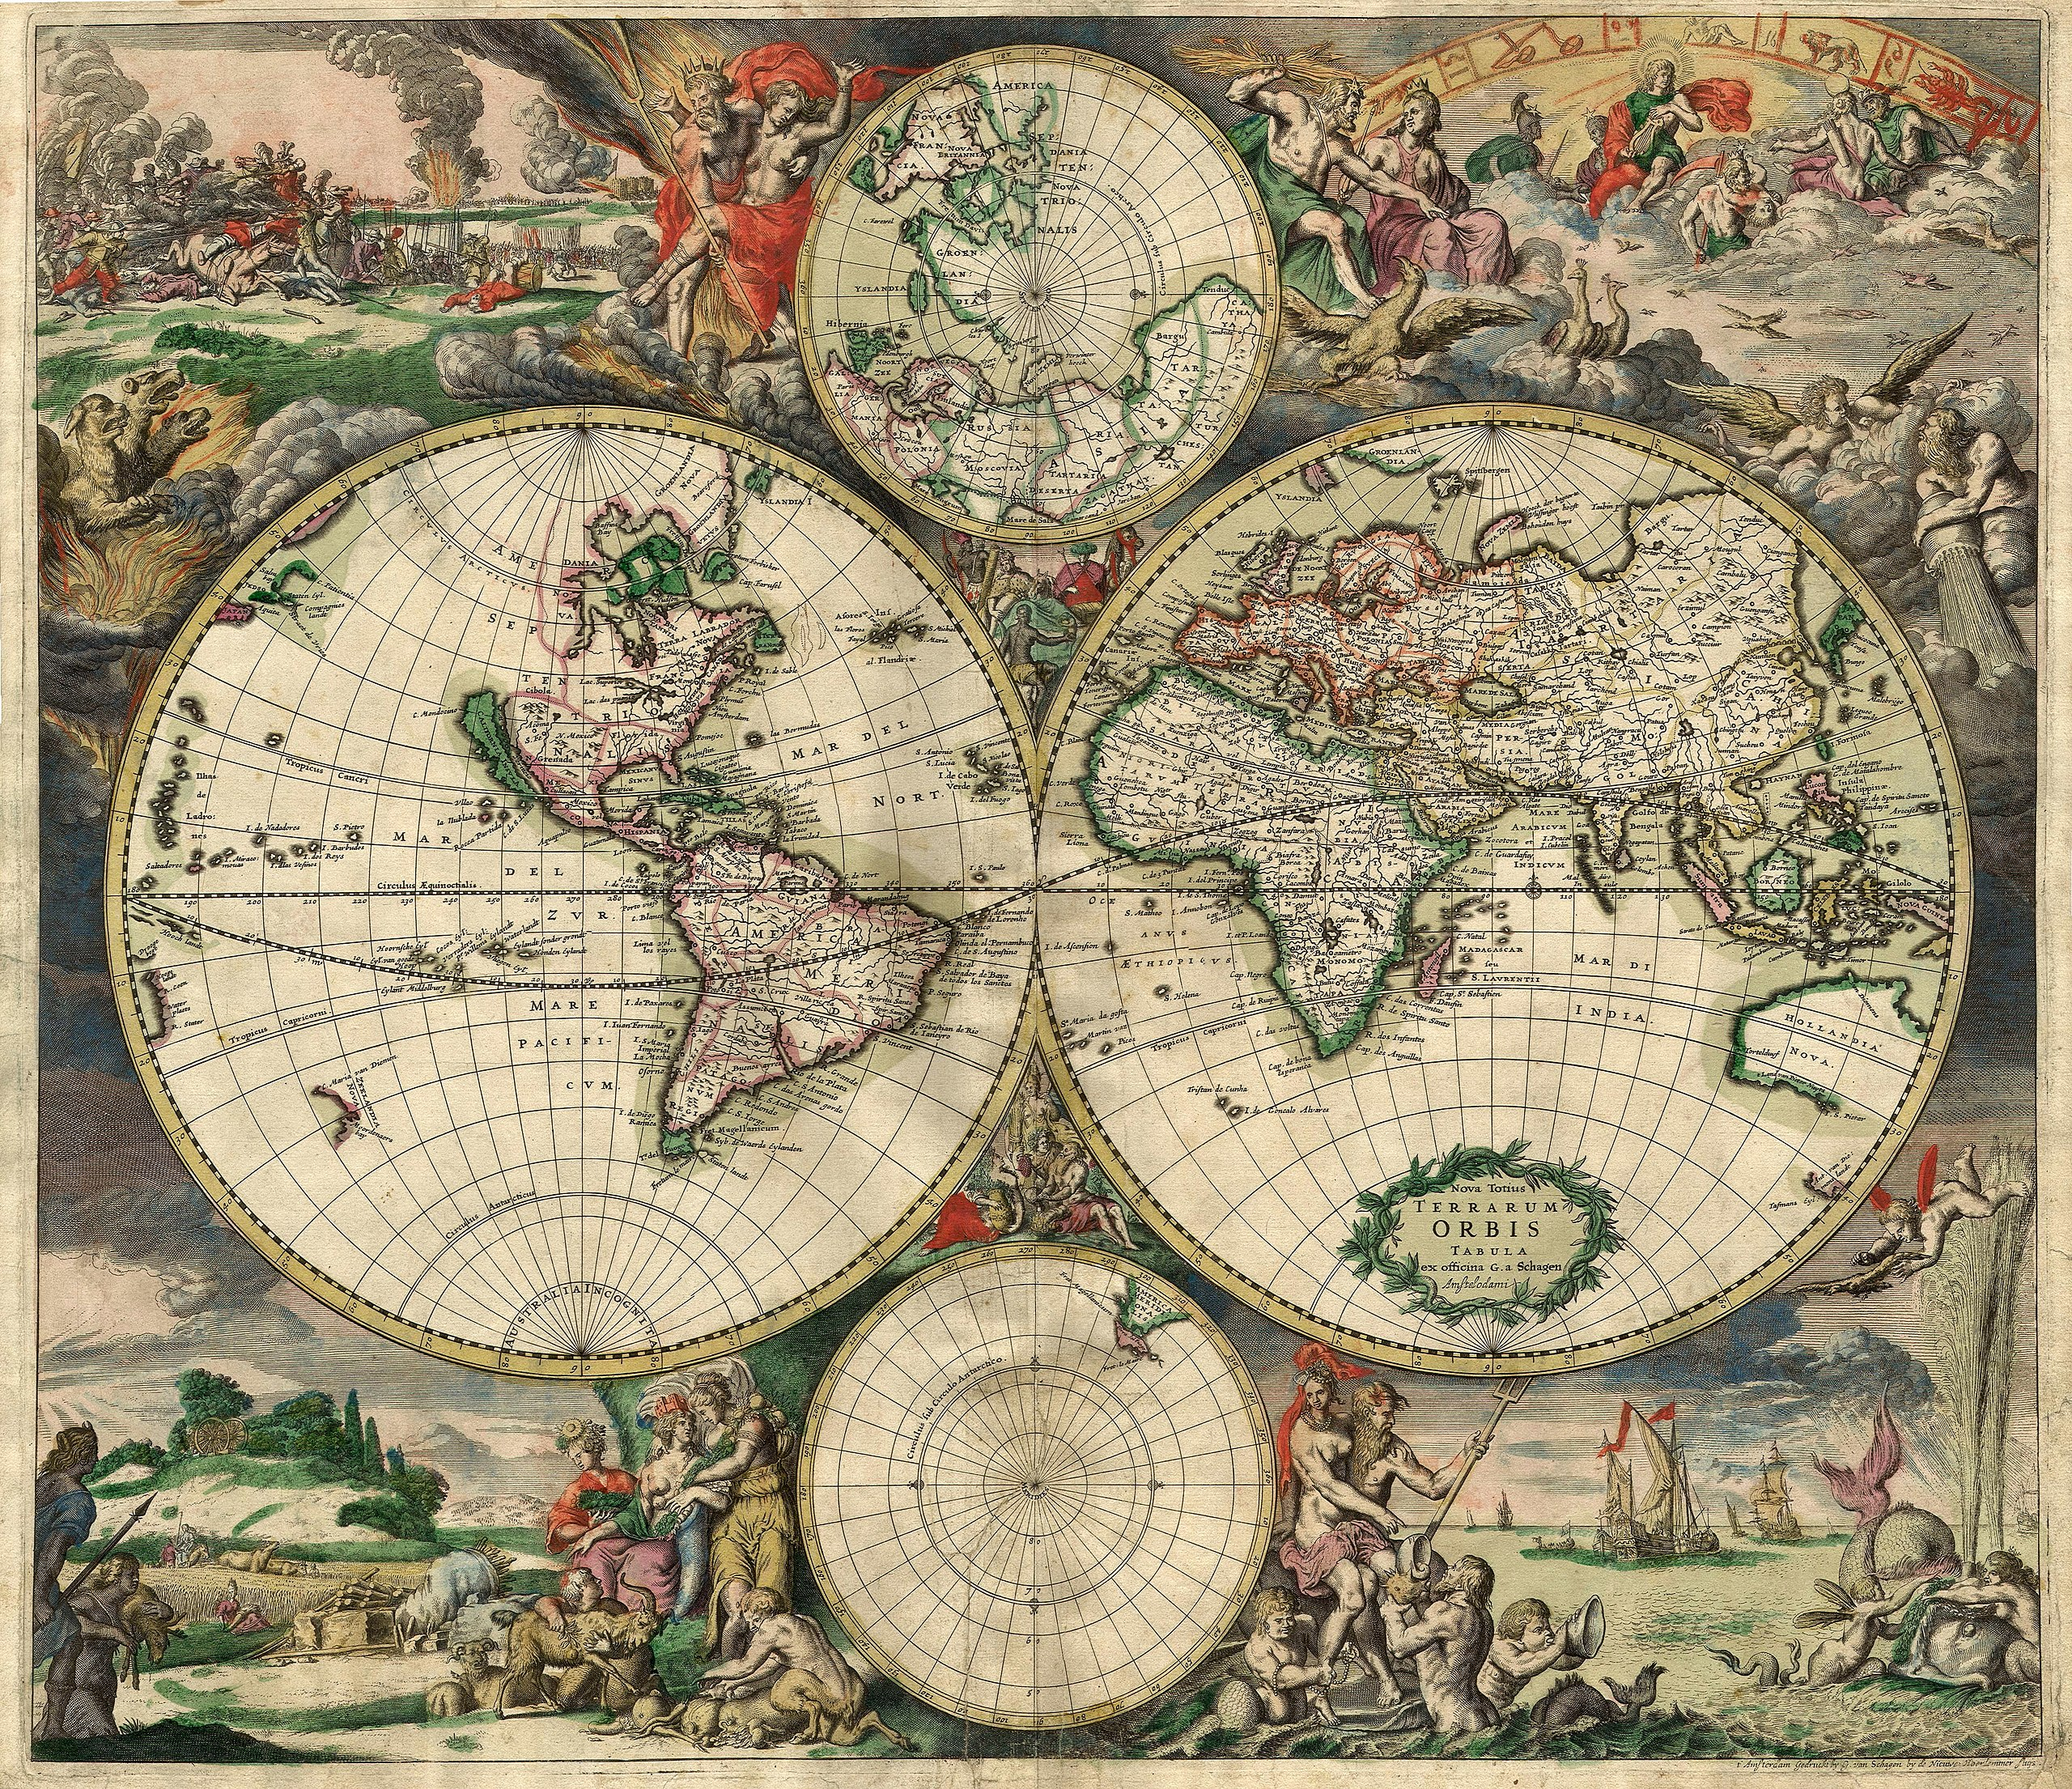
\includegraphics[width=0.8\textwidth]{images/worldmap.jpg}
	\end{center}


\end{frame}


\begin{frame}
	\frametitle{Altenative: \texttt{mmap()}}

	An alternative approach for shared memory involves the use of \texttt{mmap()}, a function nominally used to map a file into memory.

	But we can also use this for IPC!

\end{frame}


\begin{frame}[fragile]
	\frametitle{Mapping}
	\begin{lstlisting}[language=C]
void* mmap( void* address, size_t length, int protection, int flag,
   int fd, off_t offset );
\end{lstlisting}

	\texttt{address}: where you want the mapped region to go; use \texttt{NULL}.

	\texttt{length}: how many bytes to map.

	\texttt{protection}: rules for how memory can be used.

	\texttt{flag}: mode for mapping.

	\texttt{fd}: file descriptor of the file to map.

	\texttt{offset}: how far from the start of the file mapping begins.

\end{frame}


\begin{frame}
	\frametitle{Protection Flags}

	Valid values are \texttt{PROT\_NONE}, \texttt{PROT\_READ}, \texttt{PROT\_WRITE}, and \texttt{PROT\_EXECUTE}.

	They can be combined with the bitwise OR operator.

	Whatever flags you choose have to be consistent with how the file was opened with \texttt{open}.

\end{frame}


\begin{frame}
	\frametitle{\texttt{PROT\_NONE}}

	\begin{center}
		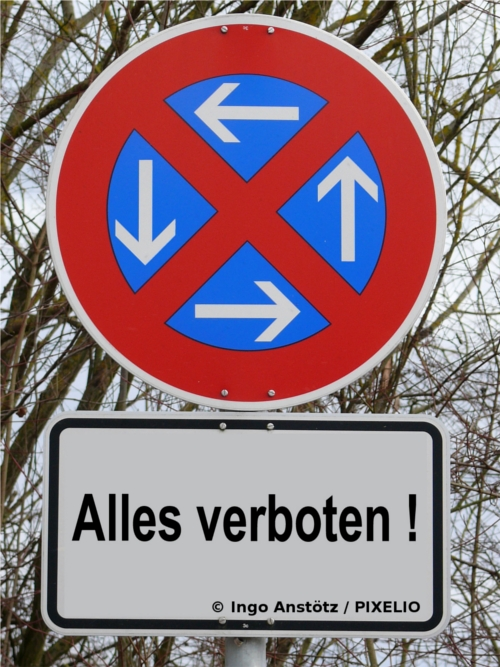
\includegraphics[width=0.45\textwidth]{images/AllesVerboten.jpg}
	\end{center}

	What's the point of \texttt{PROT\_NONE}, if all things are forbidden?

\end{frame}


\begin{frame}
	\frametitle{Flags}
	Flags can be one of two options: \texttt{MAP\_PRIVATE} or \texttt{MAP\_SHARED}.

	Private: modifications are not visible to other processes mapping the same file and not written out to the underlying file.

	Shared: modifications are visible to other processes and written out to the file... but maybe not instantly.

\end{frame}


\begin{frame}
	\frametitle{Memory Mapped File}

	\begin{center}
		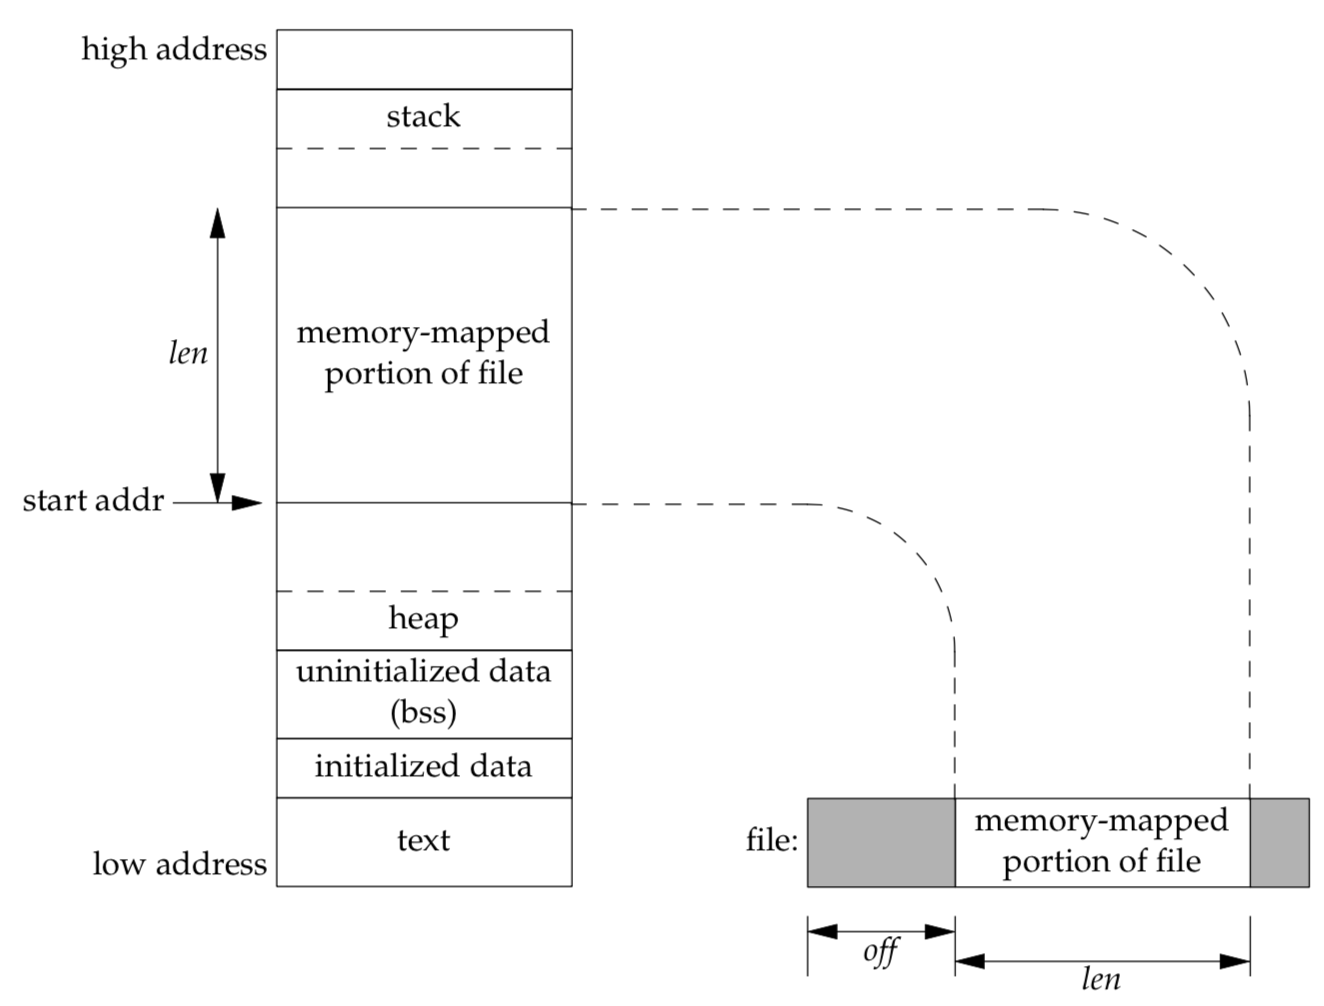
\includegraphics[width=0.9\textwidth]{images/memory-mapped-file.png}
	\end{center}

\end{frame}


\begin{frame}[fragile]
	\frametitle{Protection}

	If we wish to change the protection rules for a section, we use \texttt{mprotect}.

	\begin{lstlisting}[language=C]
int mprotect( void* address, size_t length, int prot );
\end{lstlisting}

	\texttt{address}: the memory to modify protection of.

	\texttt{length}: the size of said memory.

	\texttt{port}: the new protection rules.

\end{frame}


\begin{frame}[fragile]
	\frametitle{Synchronize}

	\begin{center}
		
\includegraphics[width=0.3\textwidth]{images/sync-icon.png}
	\end{center}

	\begin{lstlisting}[language=C]
int msync( void* address, size_t length, int flags );
\end{lstlisting}

	\texttt{address}: the memory to synchronize.

	\texttt{length}: how many bytes to synchronize.

	\texttt{flags}: mode for synchronization; use \texttt{MS\_SYNC} (blocking).

\end{frame}


\begin{frame}[fragile]
	\frametitle{Unmap}

	\begin{lstlisting}[language=C]
int munmap( void* address, size_t length );
\end{lstlisting}

	\texttt{address}: the memory to unmap.

	\texttt{length}: how many bytes to unmap.

	A segment would be unmapped automatically when a process exits, but as always it is polite to unmap it as soon as you know that you are done with it.

\end{frame}


\begin{frame}[fragile]
	\frametitle{Memory Mapping Example}

	\begin{lstlisting}[language=C]
#define _XOPEN_SOURCE
#include <stdio.h>
#include <stdlib.h>
#include <sys/shm.h>
#include <string.h>
#include <unistd.h>
#include <sys/wait.h>
#include <sys/stat.h>
#include <fcntl.h>
#include <sys/mman.h>

int main( int argc, char** argv ) { 

    int fd = open( "example.txt", O_RDWR );
    
    struct stat st; 
    stat( "example.txt", &st );
    ssize_t size = st.st_size;
    void* mapped = mmap( NULL, size, PROT_READ | PROT_WRITE, MAP_SHARED, fd, 0 );  
\end{lstlisting}
\end{frame}

\begin{frame}[fragile]
	\frametitle{Memory Mapping Example}

	\begin{lstlisting}[language=C]
    int pid = fork();
    if ( pid > 0 ) { /* Parent */
        waitpid( pid, NULL, 0 );
        printf("The new content of the file is: %s.\n", (char*) mapped);
        munmap( mapped, size );
    } else if ( pid == 0 ) { /* Child */
       memset( mapped, 0, size ); /* Erase what's there */
       sprintf( mapped, "It is now Overwritten");
       /* Ensure data is synchronized */
       msync( mapped, size, MS_SYNC );
       munmap( mapped, size );
    }

    return 0;
}
\end{lstlisting}

\end{frame}

\begin{frame}
	\frametitle{The Example is... Flawed}

	The example works acceptably in the sense that we successfully overwrite the data with the new data and the parent process sees the change.

	But things get weird if we tried to write fewer bytes than the original message.

	In general, the mapped area size cannot change.

	Linux has \texttt{mremap} but this is not portable...

	But this would be great for something like sorting an array, wouldn't it?\\
	\quad The sorted array is the same size as the input and we could share the work...

\end{frame}





\end{document}

